\documentclass[12pt]{article}
\usepackage[a3paper, portrait, left=0.1mm, right =0.1mm, top=0.1mm, bottom=0.1mm]{geometry}
\usepackage[table,xcdraw]{xcolor}
\usepackage[labelformat=empty]{caption}
\usepackage{booktabs,makecell,multirow,tabularx}
\usepackage{amssymb, amsmath} %Allows for the use of symbols and mathematical objects
\usepackage{verbatim} %Allows for the comment environment

\usepackage{tikz} %Allows for creation of images in the tikz environment
\usetikzlibrary{mindmap} %Allows the generation of fancy mindmaps
\usetikzlibrary{backgrounds} %Allows bacgrounds to be added to figures
\usetikzlibrary{shapes.geometric, arrows}



\begin{document}
\tikzstyle{background rectangle}=[top color=green, bottom color=blue!70!white] %Adds a background to the image
\tikzstyle{every annotation}=[fill=yellow, text=black, font= \small, align=left] %defines a standard annotation style

%For \path [mindmap] the following outside the tikzpicture environment is more efficient
%\tikzstyle{root concept}+=[concept color=black!80, text=white, align= center, minimum size= 10cm, anchor= north] %Defines the root concept (RC)
%\tikzstyle{level 1 concept}+=[text=white, minimum size= 8cm, level distance= 10cm] %Defines common traits in the concepts that branch from the RC 
%\tikzstyle{level 2 concept}+=[text=white, minimum size= 5cm, level distance= 5cm] %Defines common traits in the concepts that branch	
	
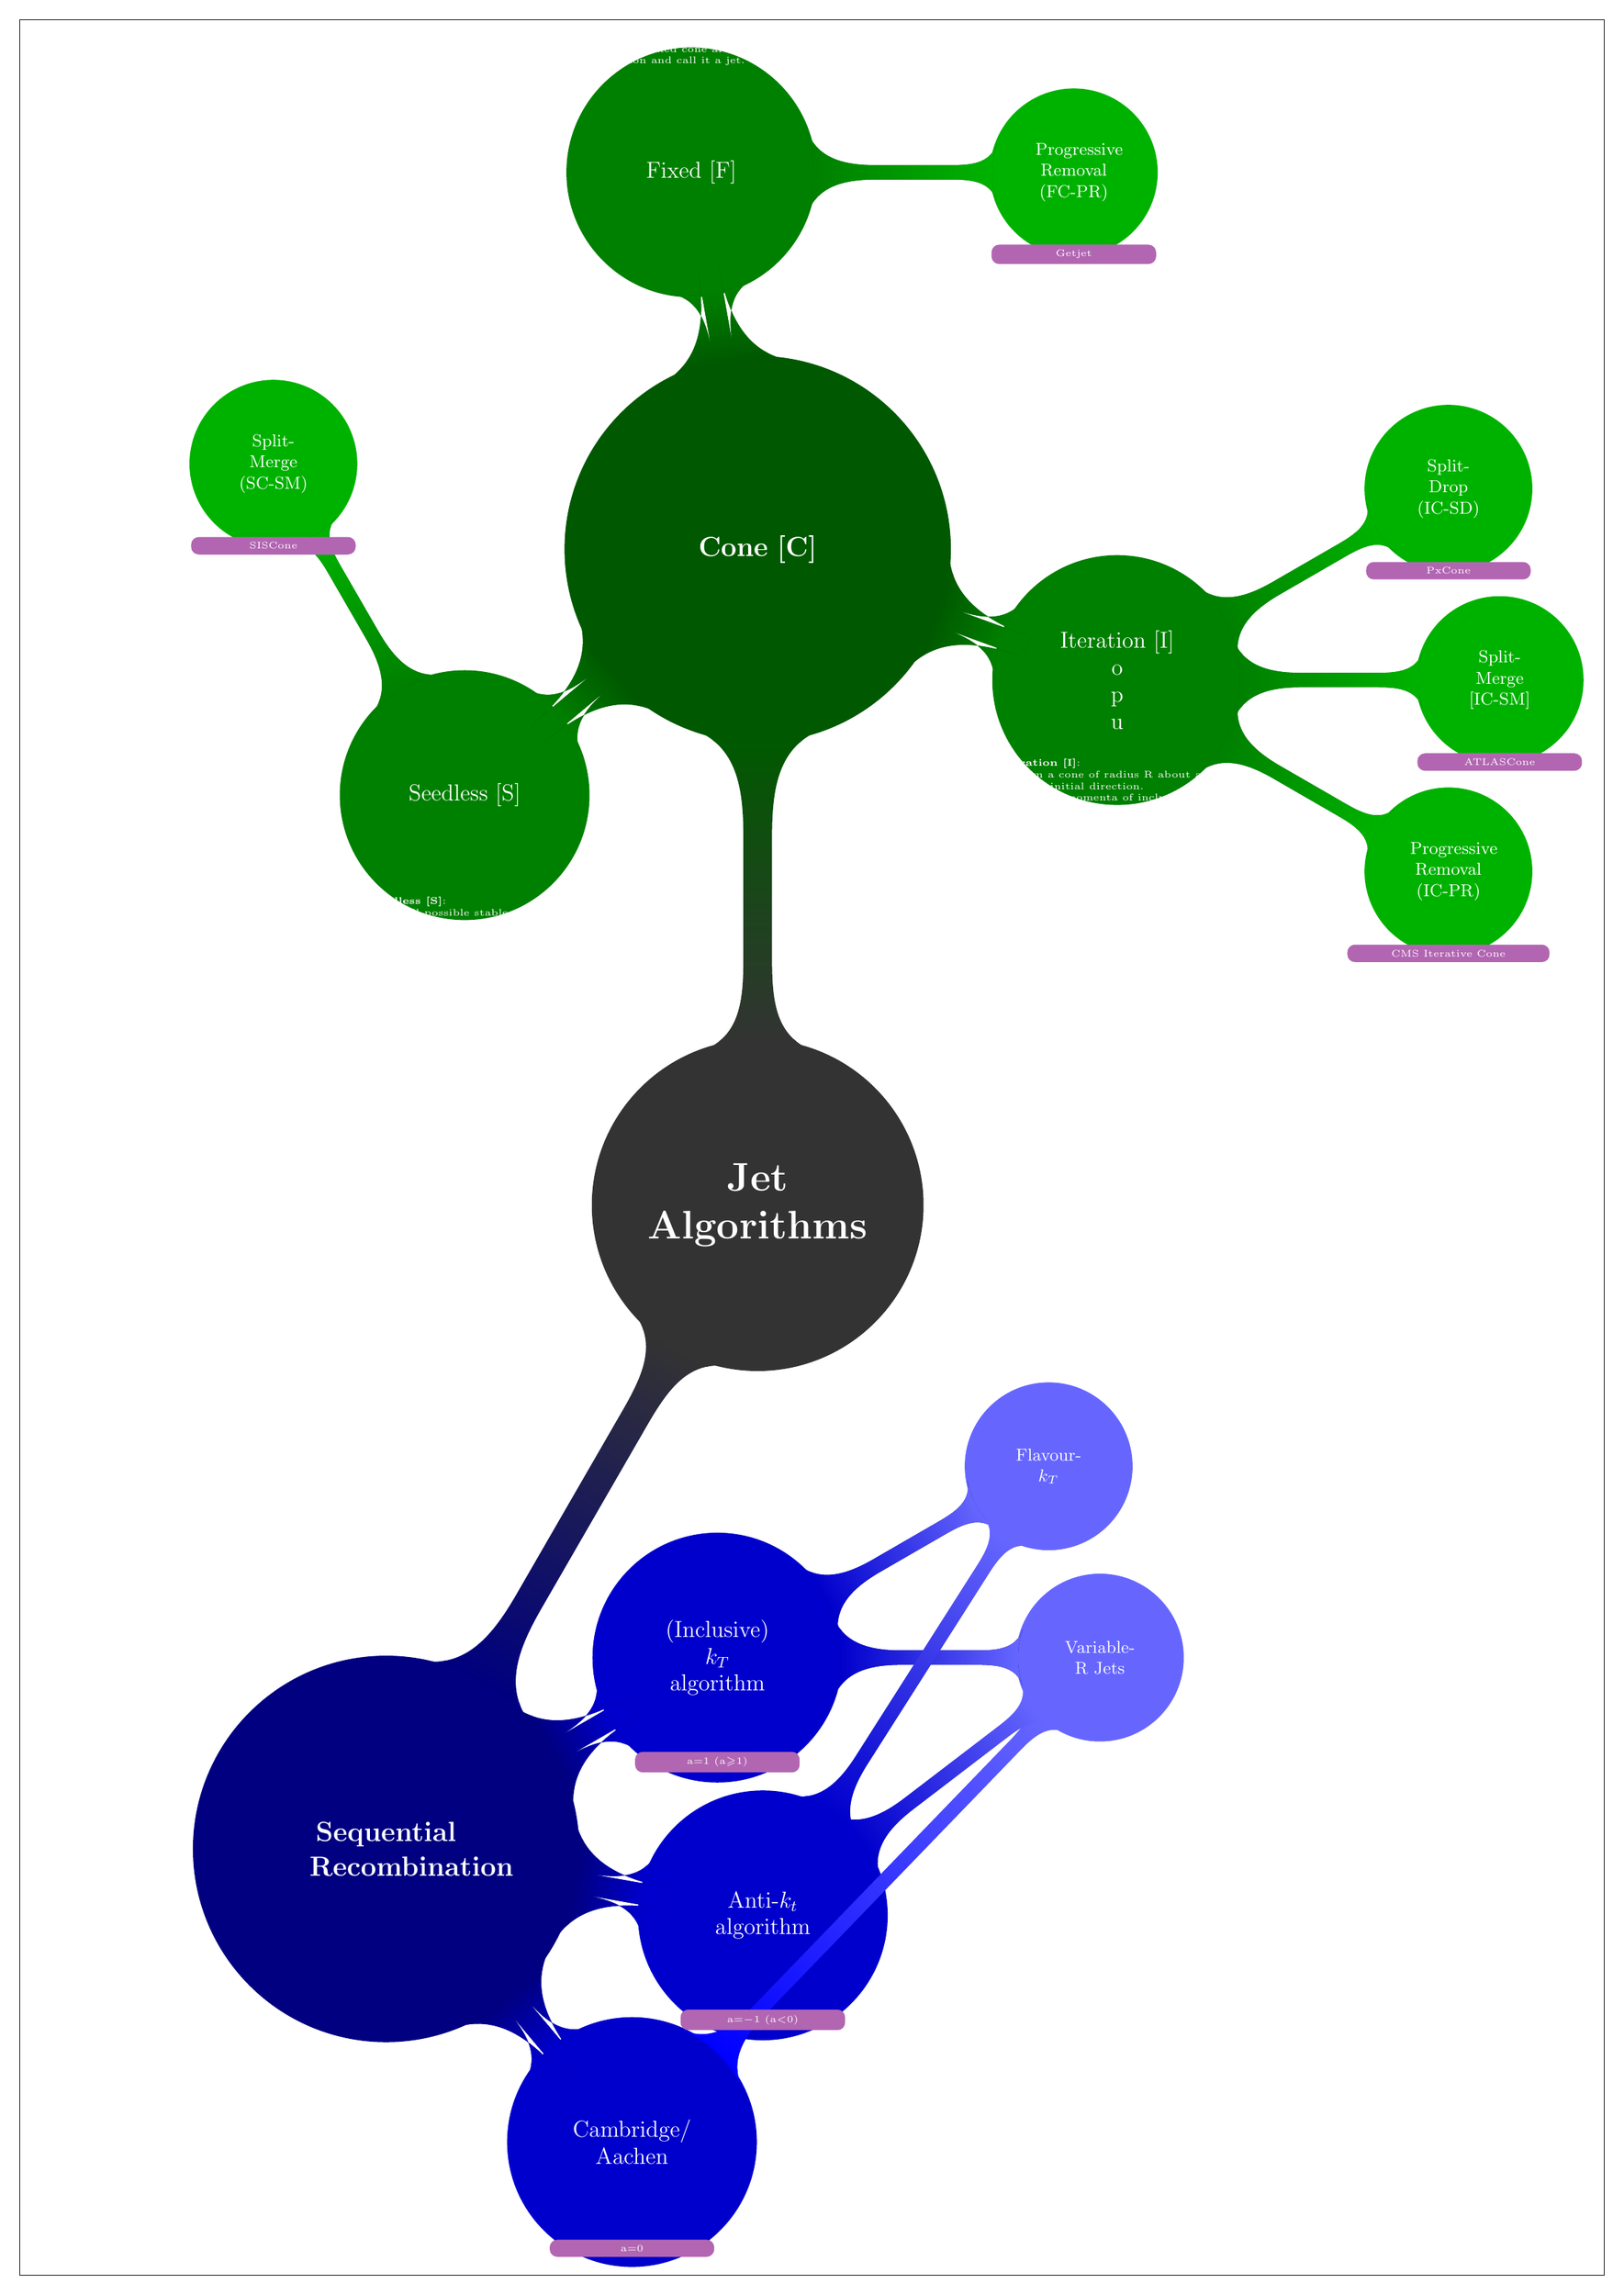
\begin{tikzpicture}[show background rectangle, large mindmap, concept color=black!80, text=white, minimum size= 6cm, font = \huge] % mindmap for A4 and huge mindmap for A2 and above 

\tikzstyle{level 1 concept}+=[text=white, minimum size= 7cm, level distance= 12cm, font = \Large] %Defines common traits in the concepts that branch from the RC (lvl1)
\tikzstyle{level 2 concept}+=[text=white, minimum size= 4.5cm, level distance= 7cm, sibling angle = 120, font = \large] %Defines common traits in the concepts that branch from lvl1 (lvl2)
\tikzstyle{level 3 concept}+=[text=white, minimum size= 3cm, level distance= 7cm, sibling angle = 30, font = \small] %Defines common traits in the concepts that branch from lvl2 (lvl3)

% ------------------------------------------------------------ CIRCLES
    	
		\node [concept](Jet Algorithms) {\textbf{Jet \\ Algorithms}} %[item, format specifics] (label name) {text content}
		child[grow=up, concept color=green!35!black]{
		node[concept, text=white] (Cone) {\textbf{Cone [C]}}
		[counterclockwise from=-20]
				child { 
				node[concept, concept color=green!50!black] (iteration) {Iteration [I] \\ o \\ p \\ u } %Stuff added to make 'Iteration' sit in the right place
				[counterclockwise from = -30]
						child{ node[concept, concept color=green!70!black] (ICPR) {Progressive \\ Removal (IC-PR)}}
						child{ node[concept, concept color=green!70!black] (ICSM) {Split-Merge [IC-SM]}}
						child{ node[concept, concept color=green!70!black] (ICSD) {Split-Drop (IC-SD)}}
				}
				child { 
				node[concept, concept color=green!50!black] (fixed) {{Fixed [F]} }
				[counterclockwise from = 0]
						child{ node[concept, concept color=green!70!black] (FCPR) {Progressive \\ Removal (FC-PR)}}	
				}							
				child { 
				node[concept, concept color=green!50!black] (seedless) {{Seedless [S]} } 
				[counterclockwise from = -240]
						child{ node[concept, concept color=green!70!black] (SCSM) {Split-Merge (SC-SM)}}
				}				
         }						
		child[grow=240, concept color=blue!50!black, level distance = 13.6cm] {
		node[concept, text=white] (SeqRec) {\textbf{Sequential \\ Recombination}}
				child [grow=30] { 
				node[concept, concept color=blue!80!black, text=white] (kt) {(Inclusive) $k_T$ \\ algorithm} 			
				[counterclockwise from = 0]
						child{ node[concept, concept color=blue!60!white] (VR) {Variable-R Jets}}				
						child{ node[concept, concept color=blue!60!white] (Flav-kt) {Flavour-$k_T$}}
				}						
				child [grow=-50] { node[concept, concept color=blue!80!black, text=white] (C/A) {Cambridge/ Aachen} }
				child [grow=-10] { node[concept, concept color=blue!80!black, text=white] (a-kt) {Anti-$k_t$ algorithm} }
		};
		
     	\path (Cone) to[circle connection bar switch color=from (green!35!black) to (green!50!black)] (fixed);     	   	
     	\path (Cone) to[circle connection bar switch color=from (green!35!black) to (green!50!black)] (seedless);		
     	\path (Cone) to[circle connection bar switch color=from (green!35!black) to (green!50!black)] (iteration);
     	\path (seedless) to[circle connection bar switch color=from (green!50!black) to (green!70!black)] (SCSM);
     	\path (fixed) to[circle connection bar switch color=from (green!50!black) to (green!70!black)] (FCPR);
     	\path (iteration) to[circle connection bar switch color=from (green!50!black) to (green!70!black)] (ICPR);
     	\path (iteration) to[circle connection bar switch color=from (green!50!black) to (green!70!black)] (ICSM);
     	\path (iteration) to[circle connection bar switch color=from (green!50!black) to (green!70!black)] (ICSD);
     	\path (SeqRec) to[circle connection bar switch color=from (blue!50!black) to (blue!80!black)] (kt);     	   	
     	\path (SeqRec) to[circle connection bar switch color=from (blue!50!black) to (blue!80!black)] (C/A);
     	\path (SeqRec) to[circle connection bar switch color=from (blue!50!black) to (blue!80!black)] (a-kt);			
     	\path (kt) to[circle connection bar switch color=from (blue!80!black) to (blue!60!white)] (VR);
     	\path (kt) to[circle connection bar switch color=from (blue!80!black) to (blue!60!white)] (Flav-kt);     	   	
     	\path (C/A) to[circle connection bar switch color=from (blue!100!black) to (blue!60!white)] (VR);
     	\path (a-kt) to[circle connection bar switch color=from (blue!80!black) to (blue!60!white)] (VR);
     	\path (a-kt) to[circle connection bar switch color=from (blue!80!black) to (blue!60!white)] (Flav-kt);
% ------------------------------------------------------------ ANNOTATIONS
		
		\node[annotation] at (fixed.north){ \textbf{Fixed [F]}:\\ Create a fixed cone around seed direction and call it a jet.};
     	\node[annotation] at (seedless.south){ \textbf{Seedless [S]}:\\ Finds all possible stable cones using a particular technique that uses no iterations or seeds.};
     	\node[annotation, text width=120] at (iteration.south){\textbf{Iteration [I]}: \\ 
     		$\bullet$ Form a cone of radius R about a seed with an initial direction. \\ 
     		$\bullet$ Sum the momenta of included particles and obtain a new seed direction. \\ 
     		$\bullet$ Repeat the process until the cone is stable.
     	};

     	\node[annotation, right, text width = 115](PR) at (FCPR.east) {\textbf{Progressive Removal [PR]:}\\ 
     		$\bullet$ Form a jet from the hardest seed. \\ 
     		$\bullet$ Remove from the event all particles in that jet. \\ 
       		$\bullet$ Repeat with the next hardest particle/tower until no particles are left above a certain threshold.
       	};
     	\node[annotation, above, text width = 250](SM) at (SCSM.north){\textbf{Split Merge [SM]}:\\ 
     		$\bullet$ From all stable cones above a threshold, 
     		merge cone pairs if more than a given fraction of the softer cones transverse momentum lies in particles that are also in the harder cone.\\ 
     		$\bullet$ Else assign the shared particles to the closer cone.
     	};
     	\node[annotation, right, text width = 90](SD) at (PR.east){\textbf{Split Drop [SD]}:\\ Works like SM but non-shared particles 
     		belonging to the softer of the two overlapping cones are dropped.
     	};
     	      	
    		\node[annotation, fill=violet!60!white, align=center, text width = 80] at (FCPR.south){Getjet};   	
     	\node[annotation, fill=violet!60!white, align=center, text width = 80] at (SCSM.south){SISCone};     	
     	\node[annotation, fill=violet!60!white, align=center] at (ICPR.south){CMS Iterative Cone};
     	\node[annotation, fill=violet!60!white, align=center, text width = 80] at (ICSM.south){ATLASCone};
     	\node[annotation, fill=violet!60!white, align=center, text width = 80] at (ICSD.south){PxCone};
     	
     	\node[annotation, above, text width = 220] at (SeqRec.north west){ \textbf{Characteristic Equations} \Large\\ 
     		$\bullet \Delta R^2_{ij} = (y_i-y_j)^2-(\phi_i-\phi_j)^2$ \\ 
     		$\bullet d_{ij}=min(p_{ti}^{2a},p_{tj}^{2a}) \frac{\Delta R^2_{ij}}{R^2}$\\ 
     		$\bullet d_{iB}=p_{ti}^{2a}$\\ 
     		$\bullet y_{ij}=\frac{2E_iE_j(1-cos\theta_{ti})}{Q^2}$
         };
         
    		\node[annotation, above, fill=violet!60!white, align=center, text width = 80] at (kt.south){a=1 (a$\geqslant$1)};   	
     	\node[annotation, above, fill=violet!60!white, align=center, text width = 80] at (C/A.south){a=0};     	
     	\node[annotation, above, fill=violet!60!white, align=center, text width = 80] at (a-kt.south){a=$-$1 (a$<$0)};  

     	\node[annotation, right, text width = 300] at (a-kt.east) {
     		$\bullet$ Work out all $d_{iB}$ and $d_{ij}$ and find the minimum of the set. \\ 
     		$\bullet$ If $d_{ij}$, recombine $j$ and $i$ into a single particle. Find the new set minimum. \\ 
     	  	$\bullet$ If $d_{iB}$, declare $i$ to be a final-state jet and remove it from particle list. Find the new set minimum. \\
     	  	$\bullet$ Continue until there are no particles left (above a given threshold)\\
     	  	-- The kT Algorithm also follows these steps.
       	};
     	\node[annotation, right, text width = 200] at (C/A.east){
     		$\bullet$ Find the pair with the smallest $\Delta R^2_{ij}$.\\ 
    		 	$\bullet$ If $\Delta R^2_{ij}$ is $<R$ replace $i$ and $j$ with their combination. Repeat.\\
    		 	$\bullet$ Else all objects are separated by $\Delta R^2_{ij} >R$ stop and call those objects jets.\\ 
     	};
     	
     	 \node[annotation, right, text width = 150] at (VR.east){
     		Redefine $d_{iB}$ and $d_{ij}$ such that they are functions of the jets' transverse momentum. \\
     		$\bullet d_{ij}=min(p_{ti}^{2a},p_{tj}^{2a})\Delta R^2_{ij}$\\ 
     		$\bullet d_{iB}=p_{ti}^{2a}$
     	};   	   	 

     	 \node[annotation, right, text width = 240] at (Flav-kt.north east){
     		Maintains the flavour of heavy quarks in a given jet by ensuring that soft quarks are combined with soft antiquarks, 
     		and attributing both to the same jet.\\
     		$y_{ij} \to y_{ik}^{(F)} = \frac{2E_iE_j(1-cos\theta_{ti})}{Q^2} \times T $
  			\begin{equation*}
  				T=
   				 \begin{cases}
     				 max(E_i^2,E_j^2), & \text{if softer of i,j is flavoured} \\
      				 min(E_i^2,E_j^2), & \text{if harder of i,j is flavoured}
   				 \end{cases}
  			\end{equation*}     	

     	};  
     	
\end{tikzpicture}

\end{document}
